\documentclass[draftcls,onecolumn]{IEEEtran}
%\documentclass[final,onecolumn]{IEEEtran}
%%%%%%%%%%%%%%%%%%%%%%%%%%%%%%%%%%%%%%%%%%%%%%%%%%%%%%%%%%%%%%%%%%%%%%%%%%%%%%%%
%                                                                              %
%                                   PREAMBLE                                   %
%                                                                              %
%%%%%%%%%%%%%%%%%%%%%%%%%%%%%%%%%%%%%%%%%%%%%%%%%%%%%%%%%%%%%%%%%%%%%%%%%%%%%%%%
%% INCLUDING THE PREAMBLE
%%%%%%%%%%%%%%%%%%%%%%%%%%%%%%%%%%%%%%%%%%%%%%%%%%%%%%%%%%%%%%%%%%%%%%%%%%%
%                                                                         %
%                                 PREAMBLE                                %
%                                                                         %
%%%%%%%%%%%%%%%%%%%%%%%%%%%%%%%%%%%%%%%%%%%%%%%%%%%%%%%%%%%%%%%%%%%%%%%%%%%

%% PACKAGES
\usepackage[margin=1in]{geometry}
\usepackage[]{lineno}
\linenumbers
\usepackage[usenames,dvipsnames]{xcolor}
\usepackage{listings,amsmath}
\usepackage{microtype,todonotes}
\usepackage{fancyvrb}
\VerbatimFootnotes

%% GRAPHICS RELATED
\usepackage{graphicx}
\usepackage[outdir=./tmp/]{epstopdf}
\graphicspath{{../images/}{./}{./tmp/}}
\DeclareGraphicsExtensions{.eps, .pdf, .jpeg, .png}

%% CPATION SETUP
\usepackage{float}
\usepackage{caption}
\usepackage{subcaption}
\captionsetup{belowskip=12pt,aboveskip=4pt}

%% HYPERLINKS
\usepackage[debug]{hyperref}

%% BIBLIOGRAPHY
\bibliographystyle{ieeetr}


%% EQUATIONS
%\numberwithin{equation}{section}

%% LISTINGS
\lstset{ %
    language=C++,
    basicstyle=\footnotesize\ttfamily,
    numbers=left,
    numberstyle=\tiny\color{gray},
    stepnumber=2,
    numbersep=5pt,
    backgroundcolor=\color{white},
    showspaces=false,
    showstringspaces=false,
    showtabs=false,
    frame=single,
    rulecolor=\color{black},
    tabsize=2,
    breaklines=true,
    breakatwhitespace=false,
    title=\lstname,
    keywordstyle=\color{blue},
    commentstyle=\color{OliveGreen},
    stringstyle=\color{orange}
}
\DeclareCaptionFont{white}{\color{white}}
\DeclareCaptionFormat{listing}{\colorbox[cmyk]{0.43, 0.35, 0.35, 0.01}{\parbox{\dimexpr\textwidth-2\fboxsep\relax}{#1#2#3}}}
\captionsetup[lstlisting]{format=listing,labelfont=white,textfont=white,singlelinecheck=false,margin=0pt,font={bf,footnotesize}}
\lstnewenvironment{code}[1][]%
{ \noindent\minipage{\linewidth}
	\lstset{#1}
}
{\endminipage}

%% USER COMMANDS
\usepackage{isotope}
\newcommand{\iso}{\isotope}
\newcommand{\figurewidth}{\textwidth}
\newcommand{\micron}{$\mu$m}


\usepackage{standalone}
\usepackage{siunitx}
\newcommand{\AngularFlux}{\Phi \left ( \vec{r},\hat{\Omega},E,t \right )}
% TO COMPILE: lmake
%%%%%%%%%%%%%%%%%%%%%%%%%%%%%%%%%%%%%%%%%%%%%%%%%%%%%%%%%%%%%%%%%%%%%%%%%%%%%%%%
%                                                                              %
%                               START OF DOCUMENT                              %
%                                                                              %
%%%%%%%%%%%%%%%%%%%%%%%%%%%%%%%%%%%%%%%%%%%%%%%%%%%%%%%%%%%%%%%%%%%%%%%%%%%%%%%%
\begin{document}

% Cover Page
\title{Optimization of the RPM8}
\author{Matthew J. Urffer}
\date{\today}

\maketitle
\begin{abstract}
Radiation portal monitors are designed to detect special nuclear material entering the country.
An optimized radition portal monitor is necessary in order to minimize the production cost, while ensuring that the detector requirments are meet.

Project Goals:
\begin{itemize}
	\item Minimize the amount of material in the RPM8
	\item Look at trade off betweens moderator, spacing, number of layers
	\item Does this depend on the film type?
\end{itemize}
\end{abstract}

\IEEEpeerreviewmaketitle

% Tables of Contents, Figures, Tables
\pagebreak
\tableofcontents
\listoftodos
\listoffigures
\listoftables
\lstlistoflistings
\pagebreak

\section{Introduction}
Radiation portal monitors are designed to detect special nuclear material entering the country.
An optimized radition portal monitor is necessary in order to minimize the production cost, while ensuring that the detector requirments are meet.
Thus, the optimization becomes constrained by the detector requirements, namely \SI{2.5}{cps\per\nano\gram\iso[252]{Cf}} while mainting a intrisinic gamma rejection ratio of \num{1.e-6}  \cite{kouzes_neutron_2010,kouzes_neutron_1999}.
The envisioned detector design consits of layers of \iso{6}[Li] neutron absorbing sheets sandwiched between layers of a thin light guide (less than \SI{5}{\milli \meter})\footnote{The spacing of \SI{5}{\milli \meter} was chosen because the maximum energy of the compton scattered electron from \iso[60]{Co} is \SI{1.08}{\mega \electronvolt}, which corresponds to a range of \SI{5}{\milli \meter} in plastic}.
Previous works has shown that this design is feasible.
 
\section{Methods}
\label{sec:Methodes}


The optimization of the films was formulated as finding the minimum of mass of \iso[6]{Li}
\subsection{MCNPX Simulations}
\label{sec:MCNPXMethods}

\subsection{1 D Transport Part}

\subsection{Multi-variate Optimization}
\label{sec:MVOptimization}


\section{Results}
\label{sec:Results}

\subsection{Simulated Geometries}

The simulated count for the detector designs is shown in Figure ~\ref{fig:SimCountRate}\todo{Change to CPS, not interactions}, with the values enumerated in Table \ref{tab:MCNPXCountRatePerMg}.
Not that this value does not include the scaling necessary to achieve the gamma discrimination. 
It is immediately obvious that as the maximum total count rate occurs when the most \iso[6]{Li} is present in the detector, this occurs when 6 assemblies are spaced \si{\centi\meter} from each other.
However, this is also the least efficient use of the \iso[6]{Li}.
The most efficient use of the neutron absorber requires the flux to be thermalized in order to have a high probability of interaction.
Thus, it is expected that 1 film per assembly spaced \SI{4}{\centi\meter} apart would have the the largest count rate per absorber mass.
However, it was observed in Figure ~\ref{fig:SimCountRate} that one film per assembly with assemblies spaced \SI{3}{\centi\meter} apart had the highest count rate per \si{\milli\gram} \iso[6]{Li}.
In both cases only 3 assemblies fit into the RPM8 module.
It is then thought that the additional reflector material with the assemblies spaced \SI{3}{\centi\meter} apart caused more neutrons to cross the last film.
\begin{figure}
    \centering
    \begin{subfigure}[b]{0.45\textwidth}
        \includegraphics[width=\textwidth]{RPM8Opt_CR.eps}
        \caption{Count Rate per \si{\nano\gram\iso[252]{Cf}}}
    \end{subfigure}%
    ~
    \begin{subfigure}[b]{0.45\textwidth}
        \includegraphics[width=\textwidth]{RPM8Opt_CRperLi.eps}
        \caption{Count Rate per nano gram \iso[252]{Cf} per \si{\milli\gram} \iso[6]{Li}}
    \end{subfigure}
    \caption{Count rate per dependence on number of assemblies and spacing of the simulated detectors. The amount of \iso[6]{Li} is not constant}
    \label{fig:SimCountRate}
\end{figure}
\begin{table}
  \caption{Count Rate per nano gram \iso[252]{Cf} per \si{\milli\gram} \iso[6]{Li} for the MCNPX simulated geometries}
	\label{tab:MCNPXCountRatePerMg}
  \centering
	\input{CountRatePerMg.dat}
\end{table}

\begin{figure}
	\centering
	\begin{subfigure}[b]{0.43\textwidth}
		\centering
		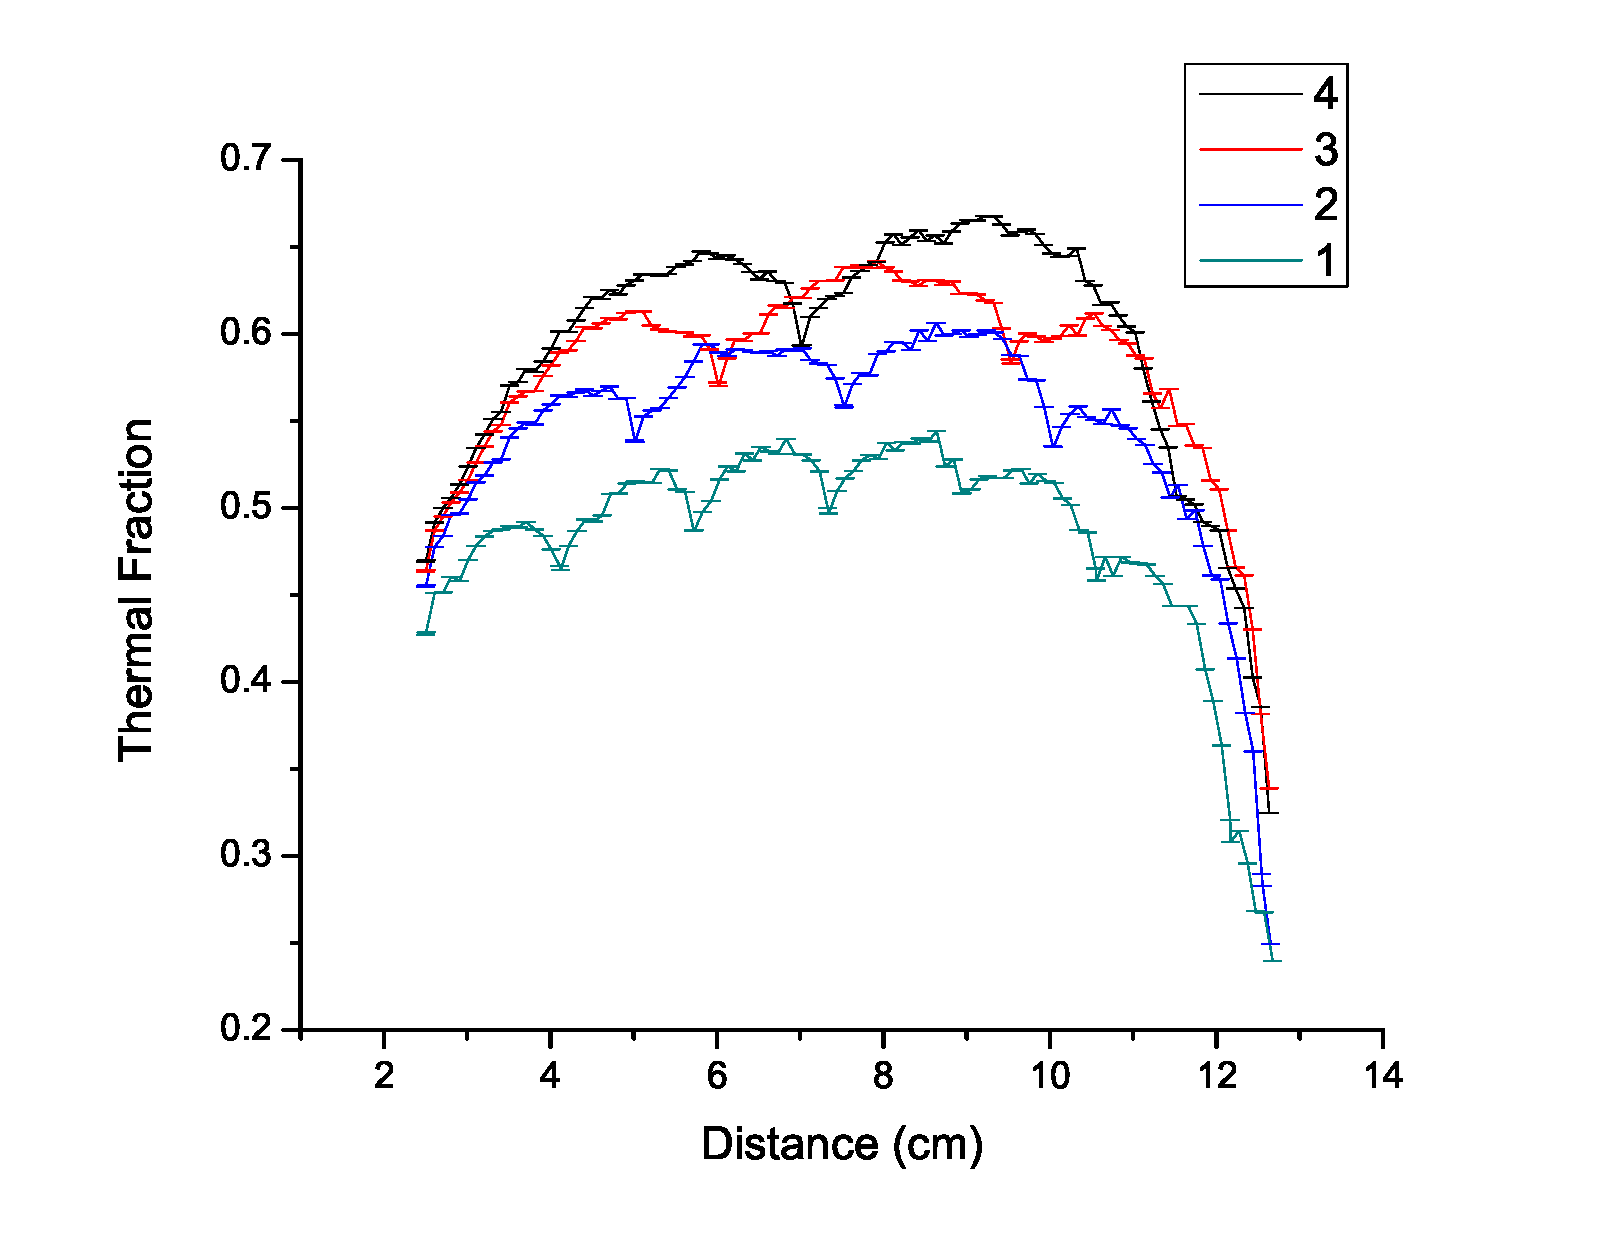
\includegraphics[width=\textwidth]{RPM8Opt_TF_1Assm.eps}
    \caption{1 Films per Assembly}
	\end{subfigure}%
	~
	\begin{subfigure}[b]{0.43\textwidth}
		\centering
		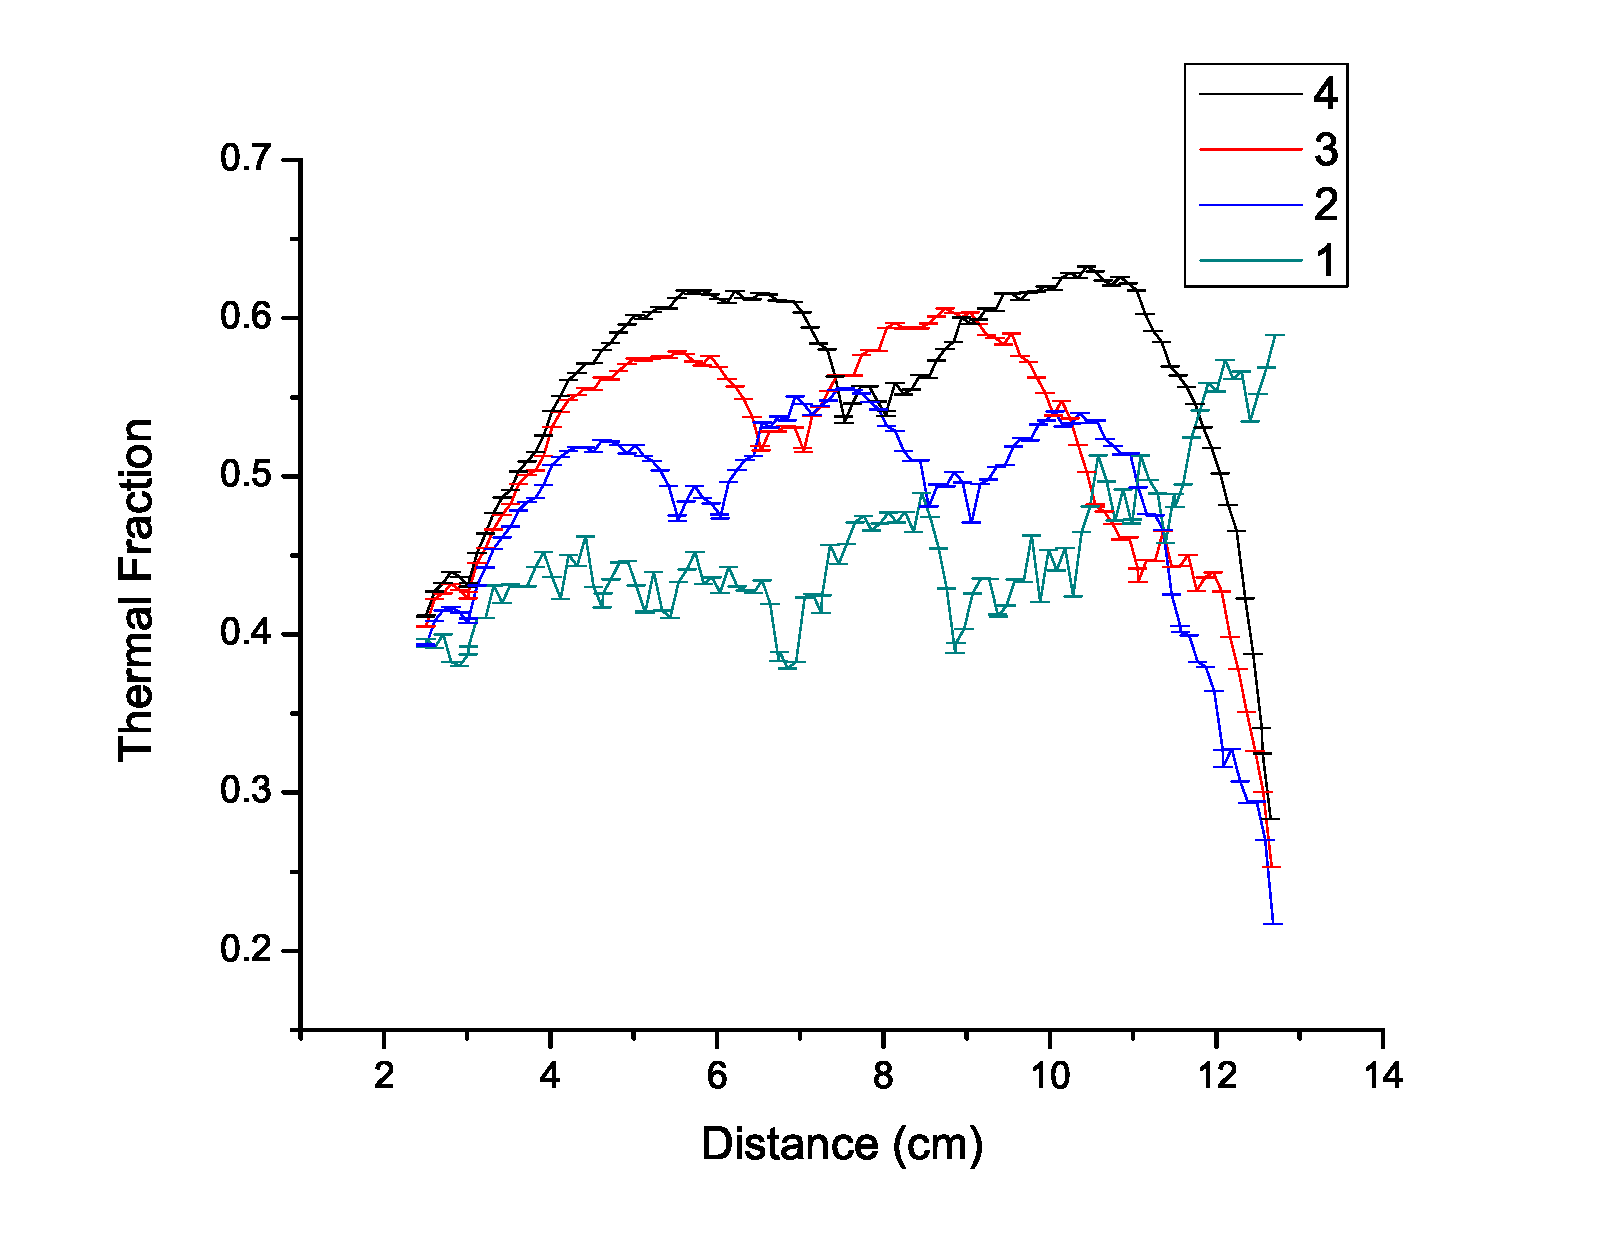
\includegraphics[width=\textwidth]{RPM8Opt_TF_2Assm.eps}
    \caption{2 Films per Assembly}
	\end{subfigure}	
	
  \begin{subfigure}[b]{0.43\textwidth}
		\centering
		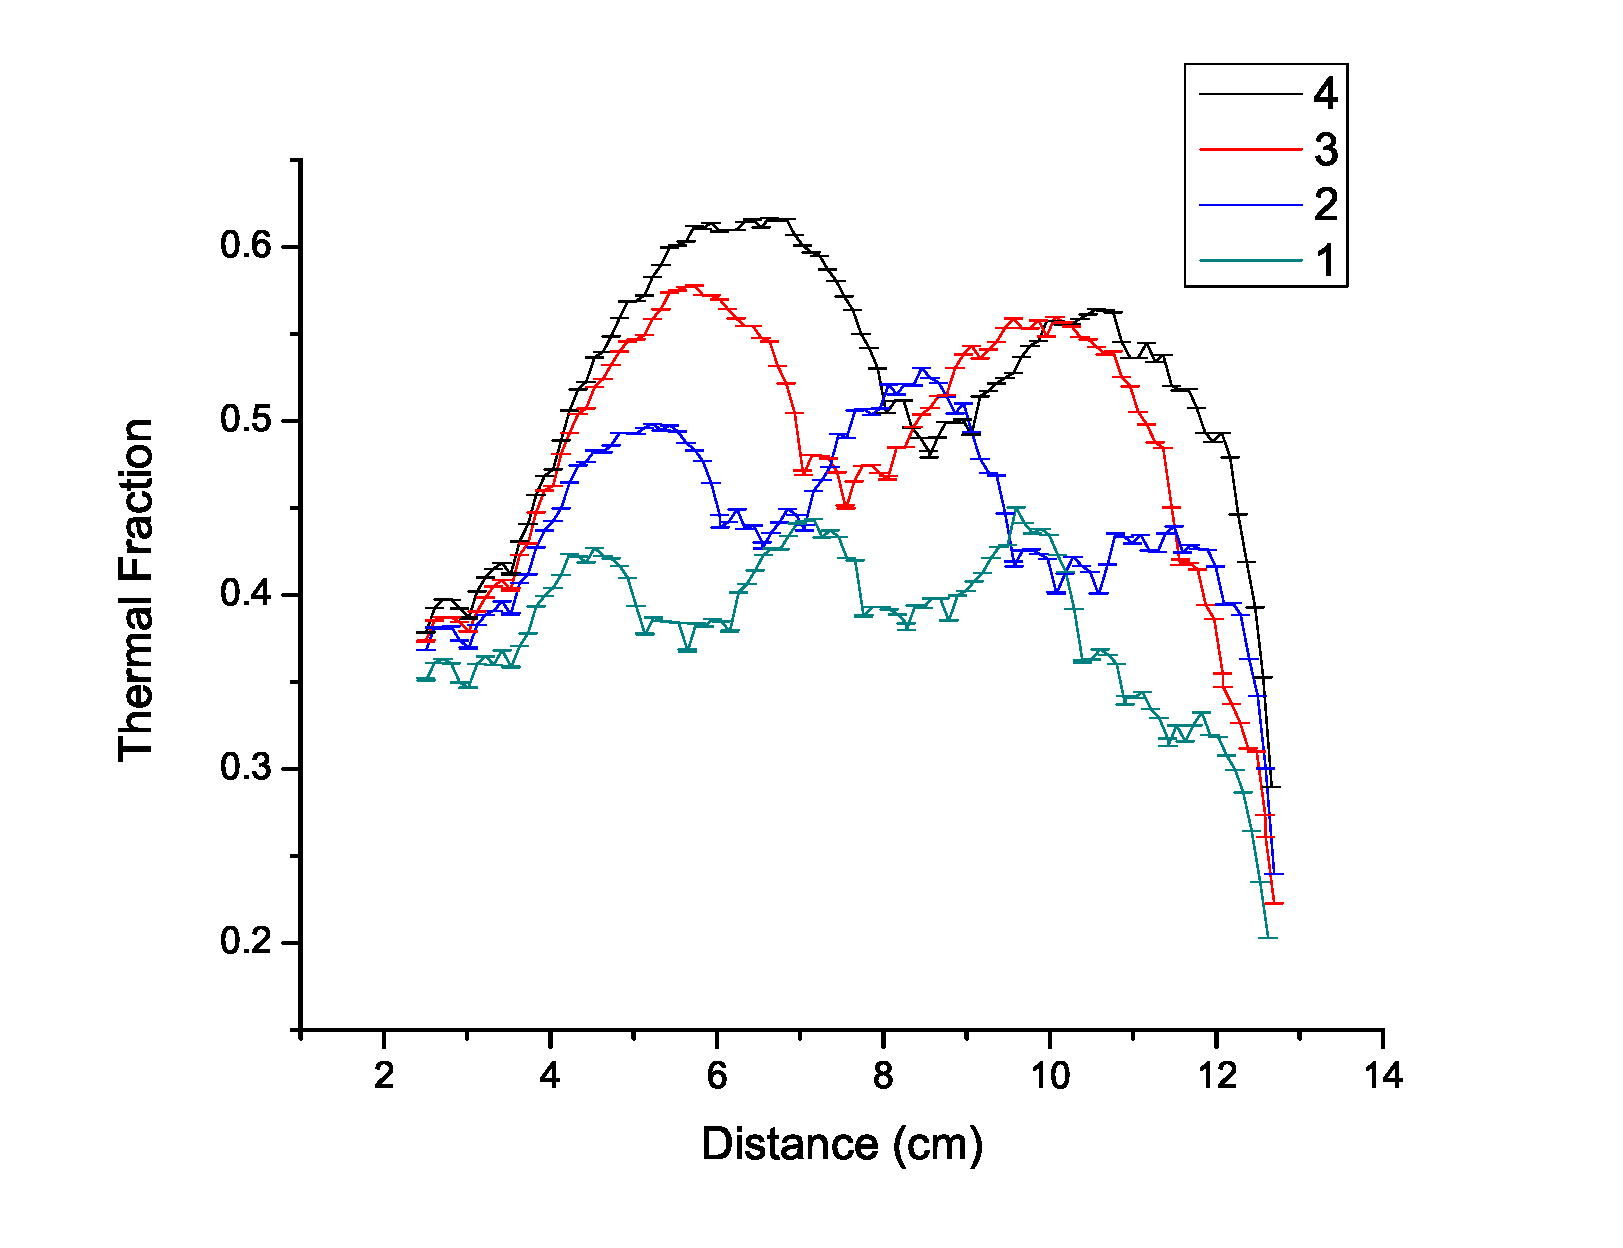
\includegraphics[width=\textwidth]{RPM8Opt_TF_3Assm.eps}
    \caption{3 Films per Assembly}
	\end{subfigure}%
	~
	\begin{subfigure}[b]{0.43\textwidth}
		\centering
		\includegraphics[width=\textwidth]{RPM8Opt_TF_4Assm.eps}
    \caption{4 Films per Assembly}
	\end{subfigure}	

	\begin{subfigure}[b]{0.43\textwidth}
		\centering
		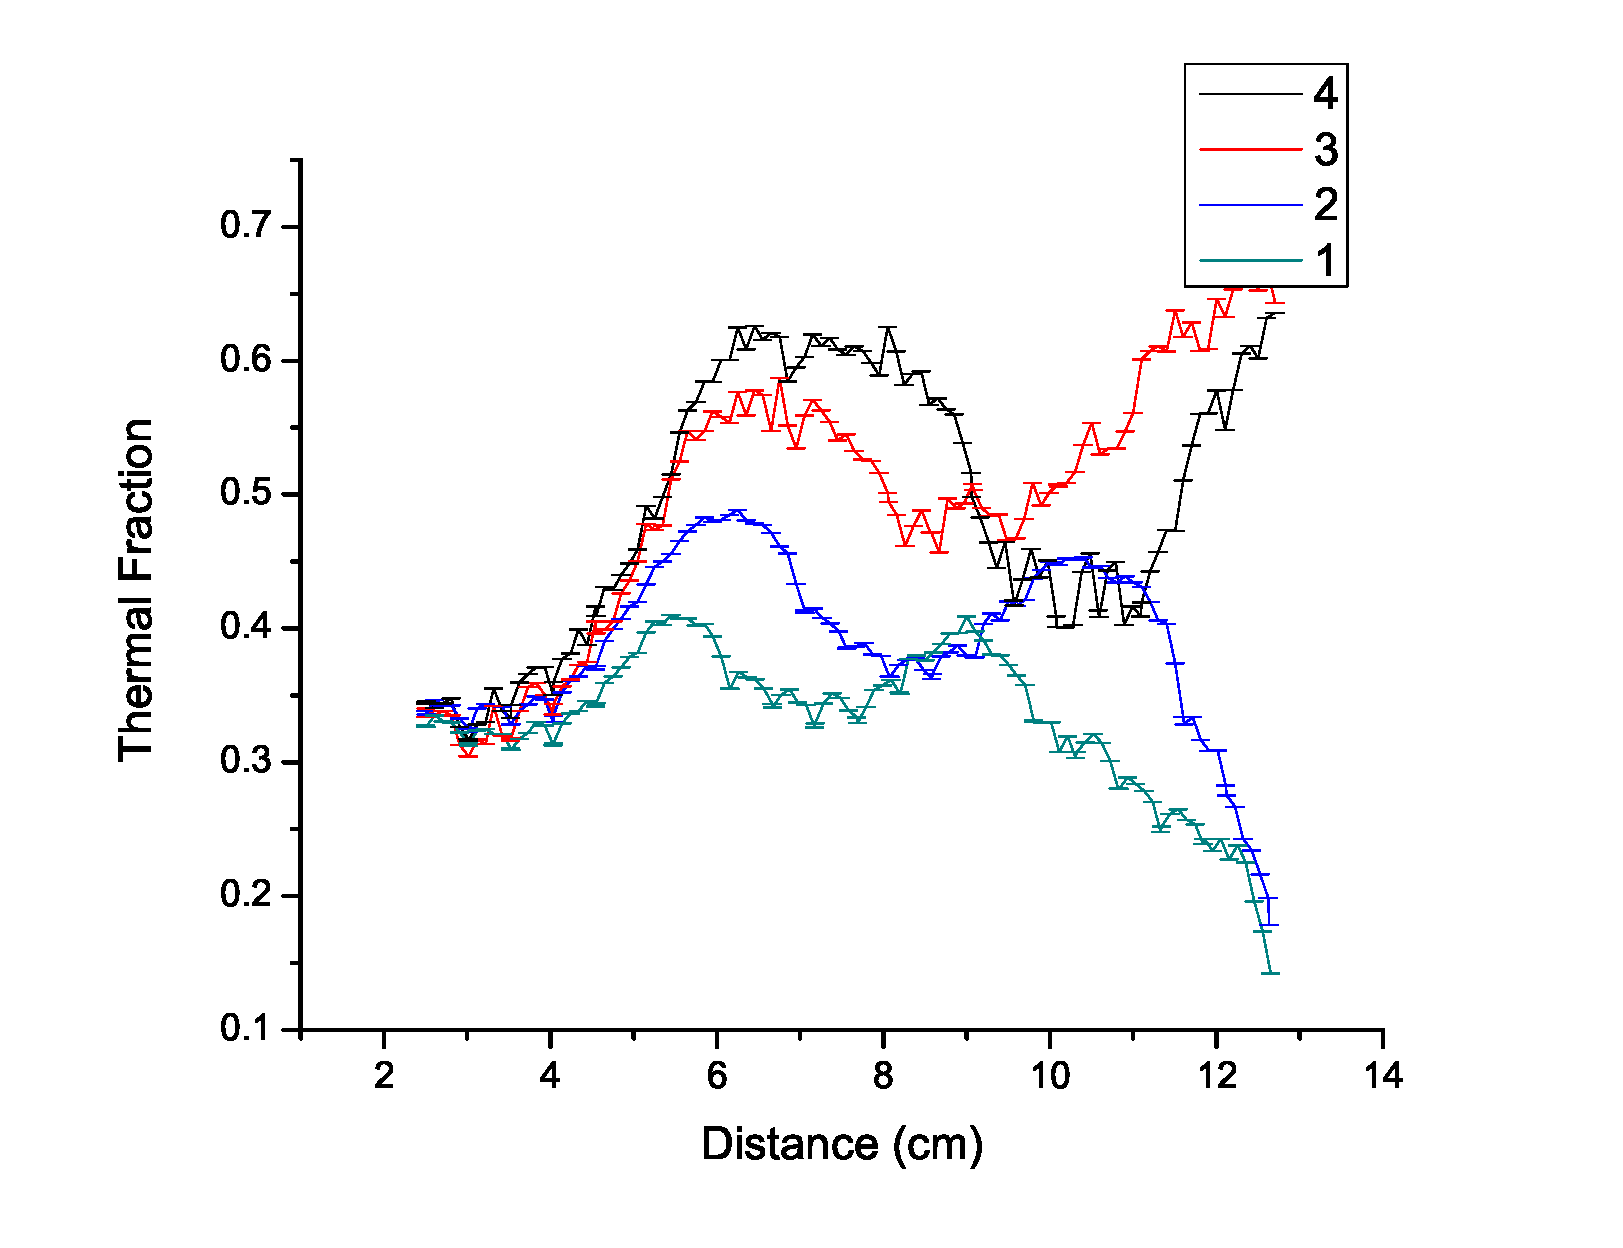
\includegraphics[width=\textwidth]{RPM8Opt_TF_5Assm.eps}
    \caption{5 Films per Assembly}
	\end{subfigure}%
	~
	\begin{subfigure}[b]{0.43\textwidth}
		\centering
		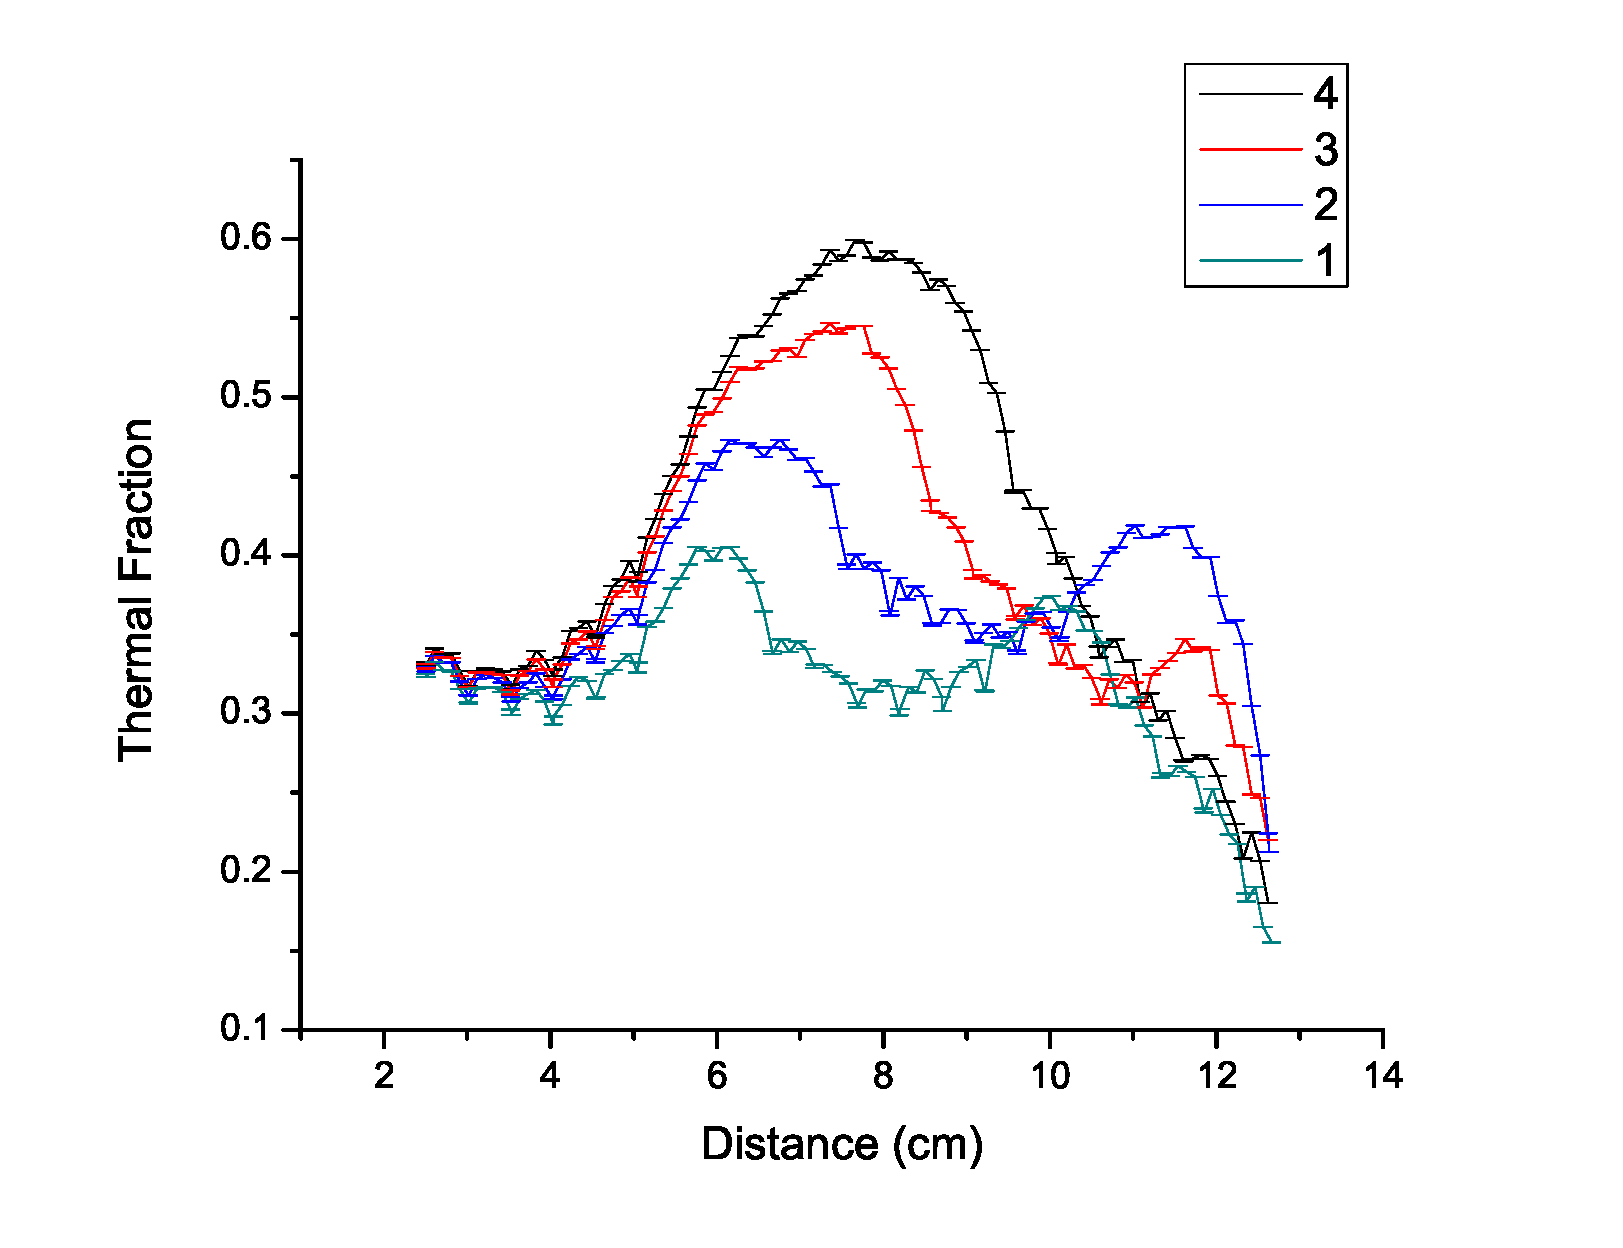
\includegraphics[width=\textwidth]{RPM8Opt_TF_6Assm.eps}
    \caption{6 Films per Assembly}
	\end{subfigure}

	\caption{Thermal Flux Profiles for Various Assemblies}
	\label{fig:ThermalFlux}
\end{figure}
\subsection{Optimized Detector Configuration}
The results of the genetic algorthim are shown below. 
Some of the search spaces were run multiple times, and what is shown is the majority vote of the algorthim on what the answer should be.
\begin{table}
  \begin{minipage}{\textwidth}
    \caption[Genomes of Optimized Geometries and Performace]{Optimized Geometries and Detector Performance\footnote{Subject to the given constraints}}
    \label{tab:GeneticOptimizedGeo}
    \centering
    \begin{tabular}{ c | c c c c}
        Genome &Assemblies&Films &Mass \iso[6]{Li} &Count Rate\\
        \hline
        \hline
        \verb+010+&1&4&16.75 &  0.175 \\
        \verb+0100+&1&4&16.75 & 0.197  \\
        \verb+01000+&1&3&12.56 & 0.230 \\
        \verb+01100+&2&6&25.13 & 0.157 \\
        \verb+0100000+&1&3&12.56& 0.229 \\
        \verb+01000000+&1&3&12.56&0.226 \\ 
        \hline
        \verb+0010000000+&1&3&& \\
        \hline
        13&2&&& \\
        26&1&&& \\
    \end{tabular}
    \end{minipage}
\end{table}

% Bibliography
\bibliography{../Zotero}

\pagebreak
\appendix
%%%%%%%%%%%%%%%%%%%%%%%%% LISTING CODE %%%%%%%%%%%%%%%%%%%%%%%%%%
\todo{Include Code Listings}

The creation of the input deck is managed by Listing ~\ref{lst:RUNDATA}.
This script uses Listing ~\ref{lst:MCNPScript} as the base MCNPX input deck.
The source cells are declared, as well as a token for which to insert the detector cells, which are dynmically generated by the python code in Listing ~\ref{lst:CreateSurfaceCell}.
The surface cells follow, along with a token for where the dynamically generated surfaces (planes) should be placed.
The run information finishes out Listing ~\ref{lst:MCNPScript}, as well as the token for placing the associated dynmically generated tallies for the detector cells the surface fluxes (Listing ~\ref{lst:CreateSurfaceCell}).
Listing ~\ref{lst:RUNDATA} also serves to submit jobs to the queue system by creating a job submission script for each run, based off of the code in Listing ~\ref{lst:QueueScript}.

Postprocessing of the output is completed with devloped python code.
Listing ~\ref{lst:ParseOutput} runs through each of the MCTAL output files generated by MCNPX and creates a MCTAL python class for each one (Listing ~\ref{lst:mctal}, ~\ref{lst:tally}).
A summary spreadsheet is generated, with additional sheets for the each of the runs.

%%%%%%%%%%%%%%%%%%%%%%%% RUN SCRIPTS %%%%%%%%%%%%%%%%%%%%%%%%%%%%%%%
\lstinputlisting[float,language=bash,caption=Run Script,label=lst:RUNDATA]{src/RUNDATA.sh}
\lstinputlisting[float,caption=Generic Assembly Input Deck,label=lst:MCNPScript]{src/SCRIPT.mcnp}
\lstinputlisting[float,language=python,caption={Surface, Cell and Tally Generator},label=lst:CreateSurfaceCell]{src/createSurfaceCells.py}
\lstinputlisting[float,language=python,caption={Merging Surface, Cells, and Tallies with base input deck},label=lst:MergeDecks]{src/mergeInputDecks.py}
\lstinputlisting[float,language=bash,caption=Queue Submission Script,label=lst:QueueScript]{src/queueRunScript.sh}
%%%%%%%%%%%%%%%%%%%%%%%%% POSTPROCESSING %%%%%%%%%%%%%%%%%%%%%%%%%%%%
\lstinputlisting[float,language=python,caption=Data Post Processing Script,label=lst:ParseOutput]{src/parseOutput.py}
\lstinputlisting[float,language=python,caption=MCTAL Class,label=lst:mctal]{src/mctal.py}
\lstinputlisting[float,language=python,caption=Tally Class,label=lst:tally,firstline=1,lastline=31]{src/tally.py}


\end{document}
